\documentclass{beamer}
\usepackage[utf8]{inputenc}
\usetheme{Madrid}
\usecolortheme{beaver}
\usepackage[labelformat=empty]{caption}
\usepackage{listings}
\usepackage{hyperref}
\usepackage[backend=biber, style=numeric, sorting=nyt]{biblatex}
\addbibresource{references.bib}
\nocite{*}


\title{DTrace}
\subtitle{…er awesome!}
\author{Carl Martin Rosenberg}
\institute{MAPS}
\date{25.02.2015}
\logo{\includegraphics[height=1.5cm]{maps_logo.eps}}

\begin{document}

\frame{\titlepage}

\begin{frame}
\frametitle{Først litt reklame…}

\begin{itemize}
    \item MAPS arrangerer programmeringskonkurranse 19.\ mars.
 \item Formatet er inspirert av \emph{Project Euler}: Finn riktig
     tekststreng!
 \item Hvordan du kommer frem til svaret (programmeringsspråk o.l.)
     er opp til deg.
 \item Det blir oppgaver for enhver smak.
 \item Bli med!
\end{itemize}

\end{frame}

\begin{frame}
\frametitle{Velkommen!}

\begin{itemize}
    \item Dette er altså et foredrag om DTrace

    \item Merk: Jeg er ikke DTrace-ekspert, men jeg tror jeg
        vet nok til å overbevise deg om at DTrace er verdt å sjekke ut!
\end{itemize}
\end{frame}
\begin{frame}
\frametitle{Velkommen!}
\begin{itemize}

    \item DTrace er en skikkelig heftig teknologi (bare vent!),
    men vanskelig å forstå uten å først forstå hvilke problemer
    det er laget for å løse.

    \item La oss derfor først ta en titt på
    hvordan software-verdenen ser ut i dag…
\end{itemize}

\end{frame}

\begin{frame}
    \frametitle{Moderne software-løsninger er \emph{systemer}}

\begin{itemize}

    \item Moderne software-løsninger er \emph{systemer}, ikke enkeltprogrammer.

    \item  Fantastisk! Man slipper å finne på hjulet på nytt!

    \item Likevel: Din egen kode er bare en bitteliten del av helheten…

    \item …og sannsynligvis den minst komplekse av dem alle.

    % \item Moderne software-utvikling drives fremover av
    %   tilgang til gjenbrukbare komponenter: operativsystemer, databaser osv.
      % Hvis du vil lage en blogg, trenger du ikke å finne opp en database, et operativsystem osv…
      % Wordpress

  %Problemet er da at løsningen du leverer til kunden består av mye mer enn
  %    koden du har skrevet selv. Faktisk er din kode kanskje den minst
  %    komplekse komponenten i løsningen…

\end{itemize}
\end{frame}

\begin{frame}
    %\frametitle{Moderne software-løsninger er systemer}
    \frametitle{Når vi utvikler komplekse systemer, trenger vi…}
\begin{itemize}

    \item Vi må kunne analysere hvordan komponentene interagerer med hverandre:
        \emph{Er det databasen eller webserveren som gjør at ting går treigt?}

    \item Vi må kunne få en viss innsikt i programmer vi enten
        \begin{enumerate}
            \item ikke selv har kildekoden til, eller
            \item ikke selv har tid og ressurser til å analysere fullstendig.
            \end{enumerate}

\end{itemize}
\end{frame}

\begin{frame}
    \frametitle{Når vi utvikler komplekse systemer, trenger vi…}
\begin{itemize}

    \item …men hva med \emph{kjørende} systemer som det er \emph{svært kostbart}
        å ta ned?

    \item  Det er ikke nok å kunne få innsikt i ting når vi sitter på våre egne
      utviklingsmaskiner.
\end{itemize}
\end{frame}

\begin{frame}
    \frametitle{Vi \emph{må} kunne få innsikt i det kjørende systemet}
\begin{itemize}
  \item Vi må raskt kunne få innsikt i det kjørende systemet…
  \item …uten at selve \emph{observasjonen av systemet} påvirker \textbf{sikkerhet} eller \textbf{ytelse}.
\end{itemize}
\end{frame}

\begin{frame}
    \frametitle{DTrace to the rescue!}

    \begin{itemize}
        \item \textbf{DTrace er laget fra bunn av for å løse disse problemene!}
    \end{itemize}

\end{frame}

\begin{frame}
    \frametitle{Om DTrace}
    \begin{itemize}

\item DTrace ble lansert av Sun Microsystems i 2005.

\item Beviste for verden at dynamisk tracing kan gjøres på en sikker måte.
    %etter flere års intenst arbeid fra noen av deres aller beste ingeniører.

\item Finnes på Mac OS X, FreeBSD, NetBSD og de fleste OpenSolaris-forks (Illumos etc.).

\item DTrace er \emph{åpen kildekode} men anses dessverre ikke for å være GPL-kompatibel.
    Dette betyr dessverre at Linux-støtten er begrenset.

\item Linux har likevel verktøy som kan gi deg det aller meste av DTrace's funksjonalitet.


    \end{itemize}

\end{frame}

\begin{frame}
    \frametitle{Nøkkelideen: Dynamisk Tracing}
    \begin{itemize}
        \item Tidligere teknologier baserte seg utelukkende på \emph{statisk} tracing.

        \item Statisk tracing kunne bare brukes til å analysere de problemene man
            antok at var viktige når man lagde programmet.

        \item Dette gjorde det ofte fristende å skape et skille mellom
              kode-under-utvikling og kode-i-produksjon
    \end{itemize}

\end{frame}

\begin{frame}
    \frametitle{Nøkkelideen: Dynamisk Tracing}
    \begin{itemize}

          \item DTrace introduserer \emph{dynamisk} tracing: DTrace kan
              observere systemet \emph{fortløende} ved å endre
         cpu-instruksjonene som ligger i minnet!

         \end{itemize}
 \end{frame}

 \begin{frame}
    \frametitle{Nøkkelideen: Dynamisk Tracing}
 \begin{itemize}

     \item Dette betyr blant annet:

         \begin{enumerate}
             \item Programmer må ikke lages observerbare for å kunne observeres:
            ‘‘Alt’’ som kjører på systemet kan observeres (bare vi er
            systematiske nok…)

        \item Programmer trenger ikke stoppes eller startes på nytt for å bli
            instrumentert (Cantrill 04)

        \item \emph{Zero overhead when not in use}: De ekstra instruksjonene som
            brukes for å observere systemet legges bare til når observasjonen
            gjøres. Systemet er ellers uendret.
         \end{enumerate}
 \end{itemize}
 \end{frame}

 \begin{frame}
    \frametitle{La oss ta en titt!}
 \begin{itemize}

     \item DTrace gir oss en observasjonspunkter for hele systemet:
         Fra alle kjørende userland-prosesser til ting i kjernen
         (scheduleren, låser mm.).

     \item Hvert observasjonspunkt representerer en \emph{hendelse},
         for eksempel hendelsen ‘‘en prosess kaller \texttt{malloc}’’.

     \item Vi bruker DTrace ved å knytte handlinger til disse hendelsene
         for å observere systemet.
 \end{itemize}
 \end{frame}

 \begin{frame}
     \frametitle{Det store bildet 1}
\begin{figure}
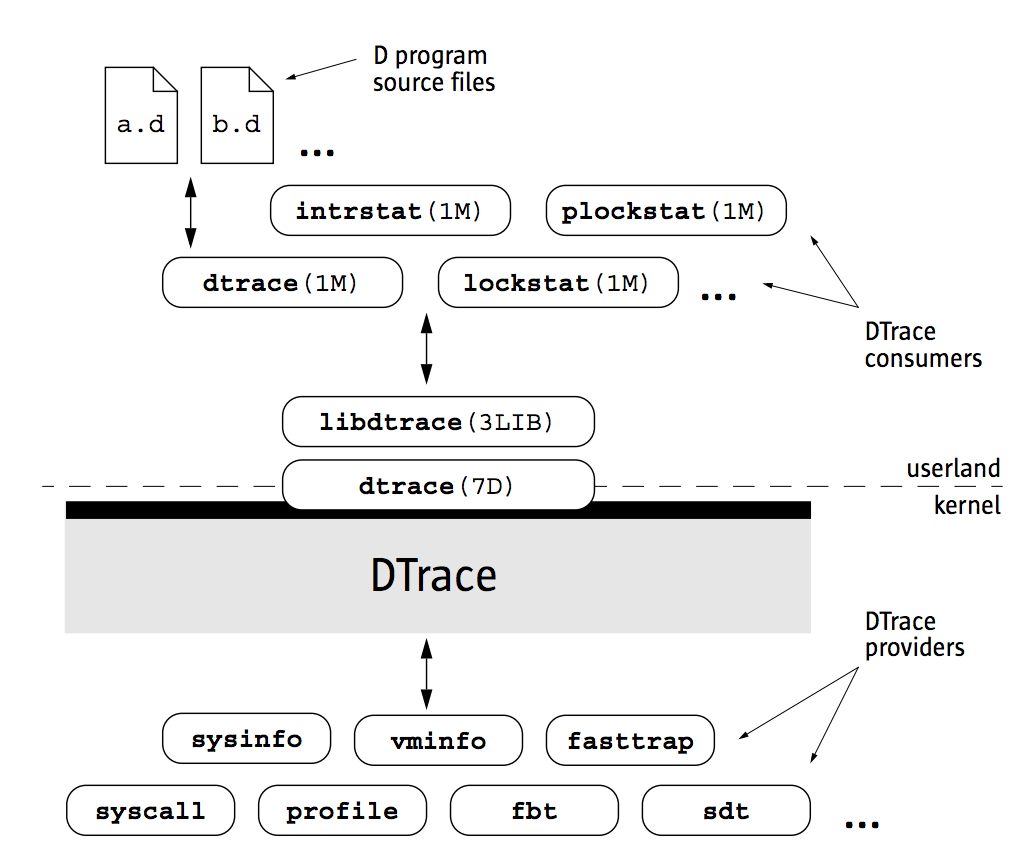
\includegraphics[scale=0.40]{architecture.png}
\caption{Fra \emph{Solaris Dynamic Tracing Guide}, side 33}
\end{figure}
 \end{frame}

 \begin{frame}
    \frametitle{Observasjonspunktene}

 \begin{itemize}

     \item Et observasjonspunkt kalles en \emph{probe}.

     \item Hvert observasjonspunkt identifiseres ved et unikt fire-tuppel:
         \texttt{<provider:module:function:name>}

    \item La oss gå dette tuppelet nærmere i sømmene…

 \end{itemize}
 \end{frame}

 \begin{frame}
    \frametitle{Providers}
    \texttt{<}\textbf{provider}\texttt{:module:function:name>}
 \begin{itemize}

     \item Providere er kjernemoduler som henter inn data på vegne av DTrace.

     \item Providere oppretter instrumenteringspunktene dynamisk.

\item Providerne iverater sikkerheten: de bestemmer hva som er trygt og hva som
      er utrygt å instrumentere. De andre komponentene i DTrace er
      ‘‘konsumenter’’ av dataene fra providerne.

  \item Systemet har providere delt inn etter tema.
\end{itemize}
\end{frame}

 \begin{frame}
    \frametitle{Providers: De vanligste}

     \begin{enumerate}
         \item \textbf{syscall}: Gir innsikt i systemkallene som operativsystemkjernen mottar.
         \item \textbf{fbt} (function boundary tracing): Gir instrumenteringspunkter for
      funksjoner i operativsystemkjernen.
  \item \textbf{proc}: Holder styr på prossessrelaterte hendelser.
  \item \textbf{sched}: Observerer scheduleren i operativsystemkjernen.
  \item \textbf{io}: Disk I/O.
  \item \textbf{tcp}: Hendelser i TCP-laget.
  \item \textbf{ip}: Hendelser i IP-stacken,  f.eks \texttt{send} og \texttt{recieve}.
  \item \textbf{pid}: Gir en egen provider for hver prosess som kjører (en slags meta-provider).
     \end{enumerate}
 \end{frame}

 \begin{frame}
    \frametitle{Providers i userland}

     \begin{itemize}
         \item I tillegg til disse kan applikasjonsutviklere lage ‘‘providere’’ for sine
    egne programmer, som eksponerer instrumenteringspunkter:
    \begin{enumerate}
        \item De fleste programmeringsspråk har en tilhørende provider
        \item Masse inflytelsesrike programmer kan kompileres til å ekseponere en 
            DTrace-provider: PostgreSQL, Node.js, Apache mm.
        \item Du kan lage dine egne (statiske) instrumenteringspunkter
        og være en provider for ditt eget program!
    \end{enumerate}
     \end{itemize}
 \end{frame}

 \begin{frame}
    \frametitle{Moduler}
    \texttt{<provider:}\textbf{module}\texttt{:function:name>}

     \begin{itemize}

         \item Hvis instrumenteringspunktet ligger i en kjernemodul, vil
    navnet på denne kjernemodulen være module-delen av tuppelet

     \begin{itemize}
         \item På FreeBSD med ZFS-filsystemet kan module være \texttt{ZFS}.
     \end{itemize}
     \end{itemize}
 \end{frame}

 \begin{frame}
     \frametitle{Moduler (forts.)}

     \begin{itemize}
         \item Hvis instrumenteringspunktet ligger i userland og er knyttet til
    et delt bibliotek, vil dette stå i module-feltet.

    \item \emph{Eksempel}: På mitt system er python-instrumenteringspunktene knyttet
        til python-modulen.

    \item  De fleste instrumenteringspunkter er ikke knyttet til en bestemt modul.
        I så fall kan vi sette en * (wildcard) i module-feltet eller bare la det stå tomt.
     \end{itemize}
 \end{frame}

 \begin{frame}
     \frametitle{Funksjoner}
     \texttt{<provider:module:}\textbf{function}\texttt{:name>}

     \begin{itemize}

         \item Hvis instrumenteringspunktet er knyttet til et faktisk funksjonssymbol
    (for eksempel \texttt{malloc}), vil dette stå på funksjonsplassen.

        \item I likhet med module er det ikke nødvendigvis slik at alle
      instrumenteringspunkter har et funksjonsfelt.

        \item Dersom et instrumenteringspunkt er knyttet til en modul
    og en funksjon, kaller vi dette en ‘‘anchored probe’’. Hvis
    ikke er den ‘‘unanchored‘‘ (Solaris Dynamic Tracing Guide).
     \end{itemize}
 \end{frame}

 \begin{frame}
     \frametitle{Name}
     \texttt{<provider:module:function:}\textbf{name}\texttt{>}

    \begin{itemize}
        \item \texttt{Name} er et felt som skal formidle hva instrumenteringspunktet er til.

        \item \texttt{Name} vil ofte være enten \texttt{BEGIN} eller \texttt{END}, korresponderende
    til henholdsvis når man går inn eller ut av en gitt funksjon.

\item \texttt{Name} kan også være mer domenespesifikt, for eksempel \texttt{acquire}, \texttt{spin}
    og \texttt{block} for en bestemt lås.

\end{itemize}
 \end{frame}

 \begin{frame}
     \frametitle{Det store bildet 2}
\begin{figure}
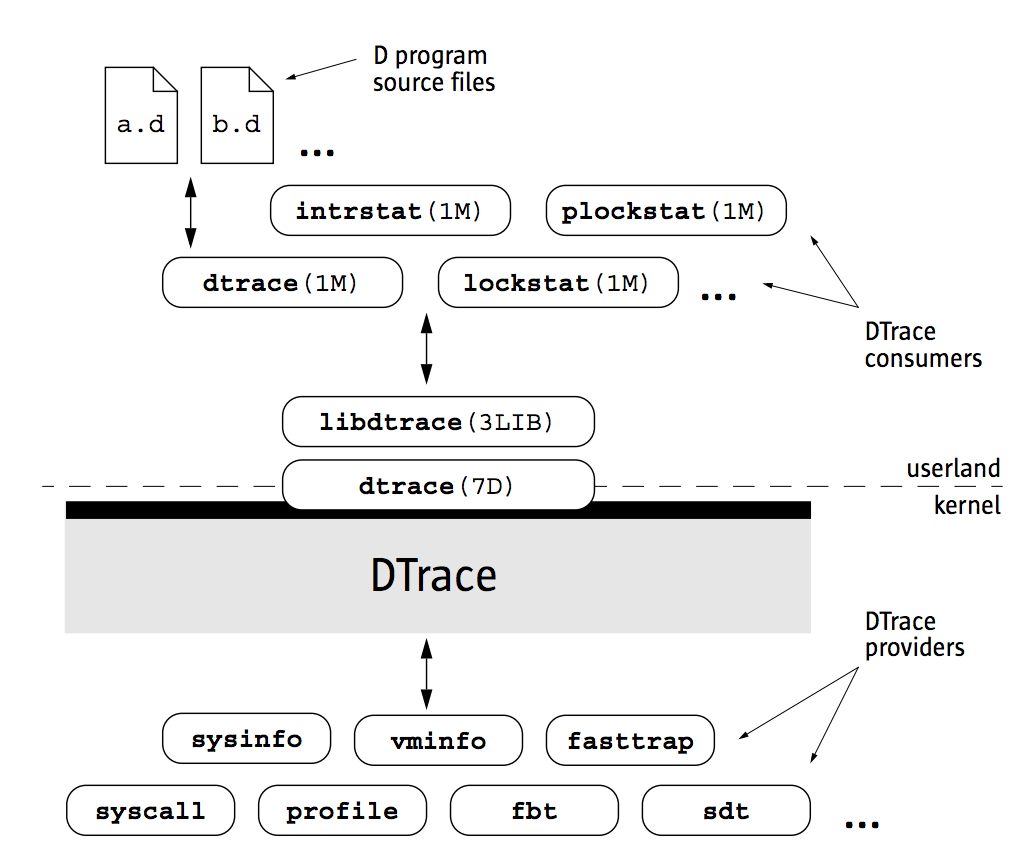
\includegraphics[scale=0.40]{architecture.png}
\caption{Fra \emph{Solaris Dynamic Tracing Guide}, side 33}
\end{figure}
 \end{frame}

 \begin{frame}
     \frametitle{D scripts}
\begin{enumerate}

    \item Hvis vi bare sier hvilke instrumenteringspunkter vi er interessert i
      og ikke oppgir en action-block, listes bare de instrumenteringspunktene
      som fyres.

  \item Så hva kan vi egentlig gjøre i action-blokken? Ganske mye!

\end{enumerate}
 \end{frame}

 \begin{frame}
     \frametitle{Actions 101}
\begin{enumerate}

\item Det mest åpenbare vi kan gjøre er å printe noe til skjermen
    når en hendelse inntreffer.

\item Dette kan vi gjøre mer sofistikert, med å bruke innebygde
    variabler, som \texttt{execname}, \texttt{pid}, \texttt{timestamp} osv.

\item Med disse enkle byggestenene kan vi til og med inspisere hvilke
    argumenter funksjoner blir kalt med!

\end{enumerate}
 \end{frame}

 \begin{frame}
     \frametitle{Actions: Innebygde funksjoner}

\begin{enumerate}
    \item Vi kan gå enda lenger…

    \item La oss finne ut filnavn som programmene på systemet forsøker å åpne
        med systemkallet \texttt{open}!

\item Kult, men blir det ikke veldig mye data?

\item Vi har to verktøy for å filtrere og fortolke datamengden:
    \emph{aggregeringer} og \emph{predikater}.

\end{enumerate}
 \end{frame}

 \begin{frame}
     \frametitle{Actions: Aggregeringer}
     \begin{itemize}
 \item Vi kan bruke aggregeringer for å få mere konsise statistikker.

 \item Det finnes adskillig mer sofistikerte aggregeringer i \texttt{count()},
     men det rekker jeg ikke gå inn på.
     \end{itemize}
 \end{frame}

\begin{frame}
     \frametitle{Predikater}
     \begin{itemize}
         \item Vi kan bruke predikater til å filtrere \emph{før} vi gjør
             actions.
         \item Sammenligningene fungerer som i \texttt{C}.
     \end{itemize}
\end{frame}
\begin{frame}
\frametitle{Hvordan det føles}
\begin{figure}
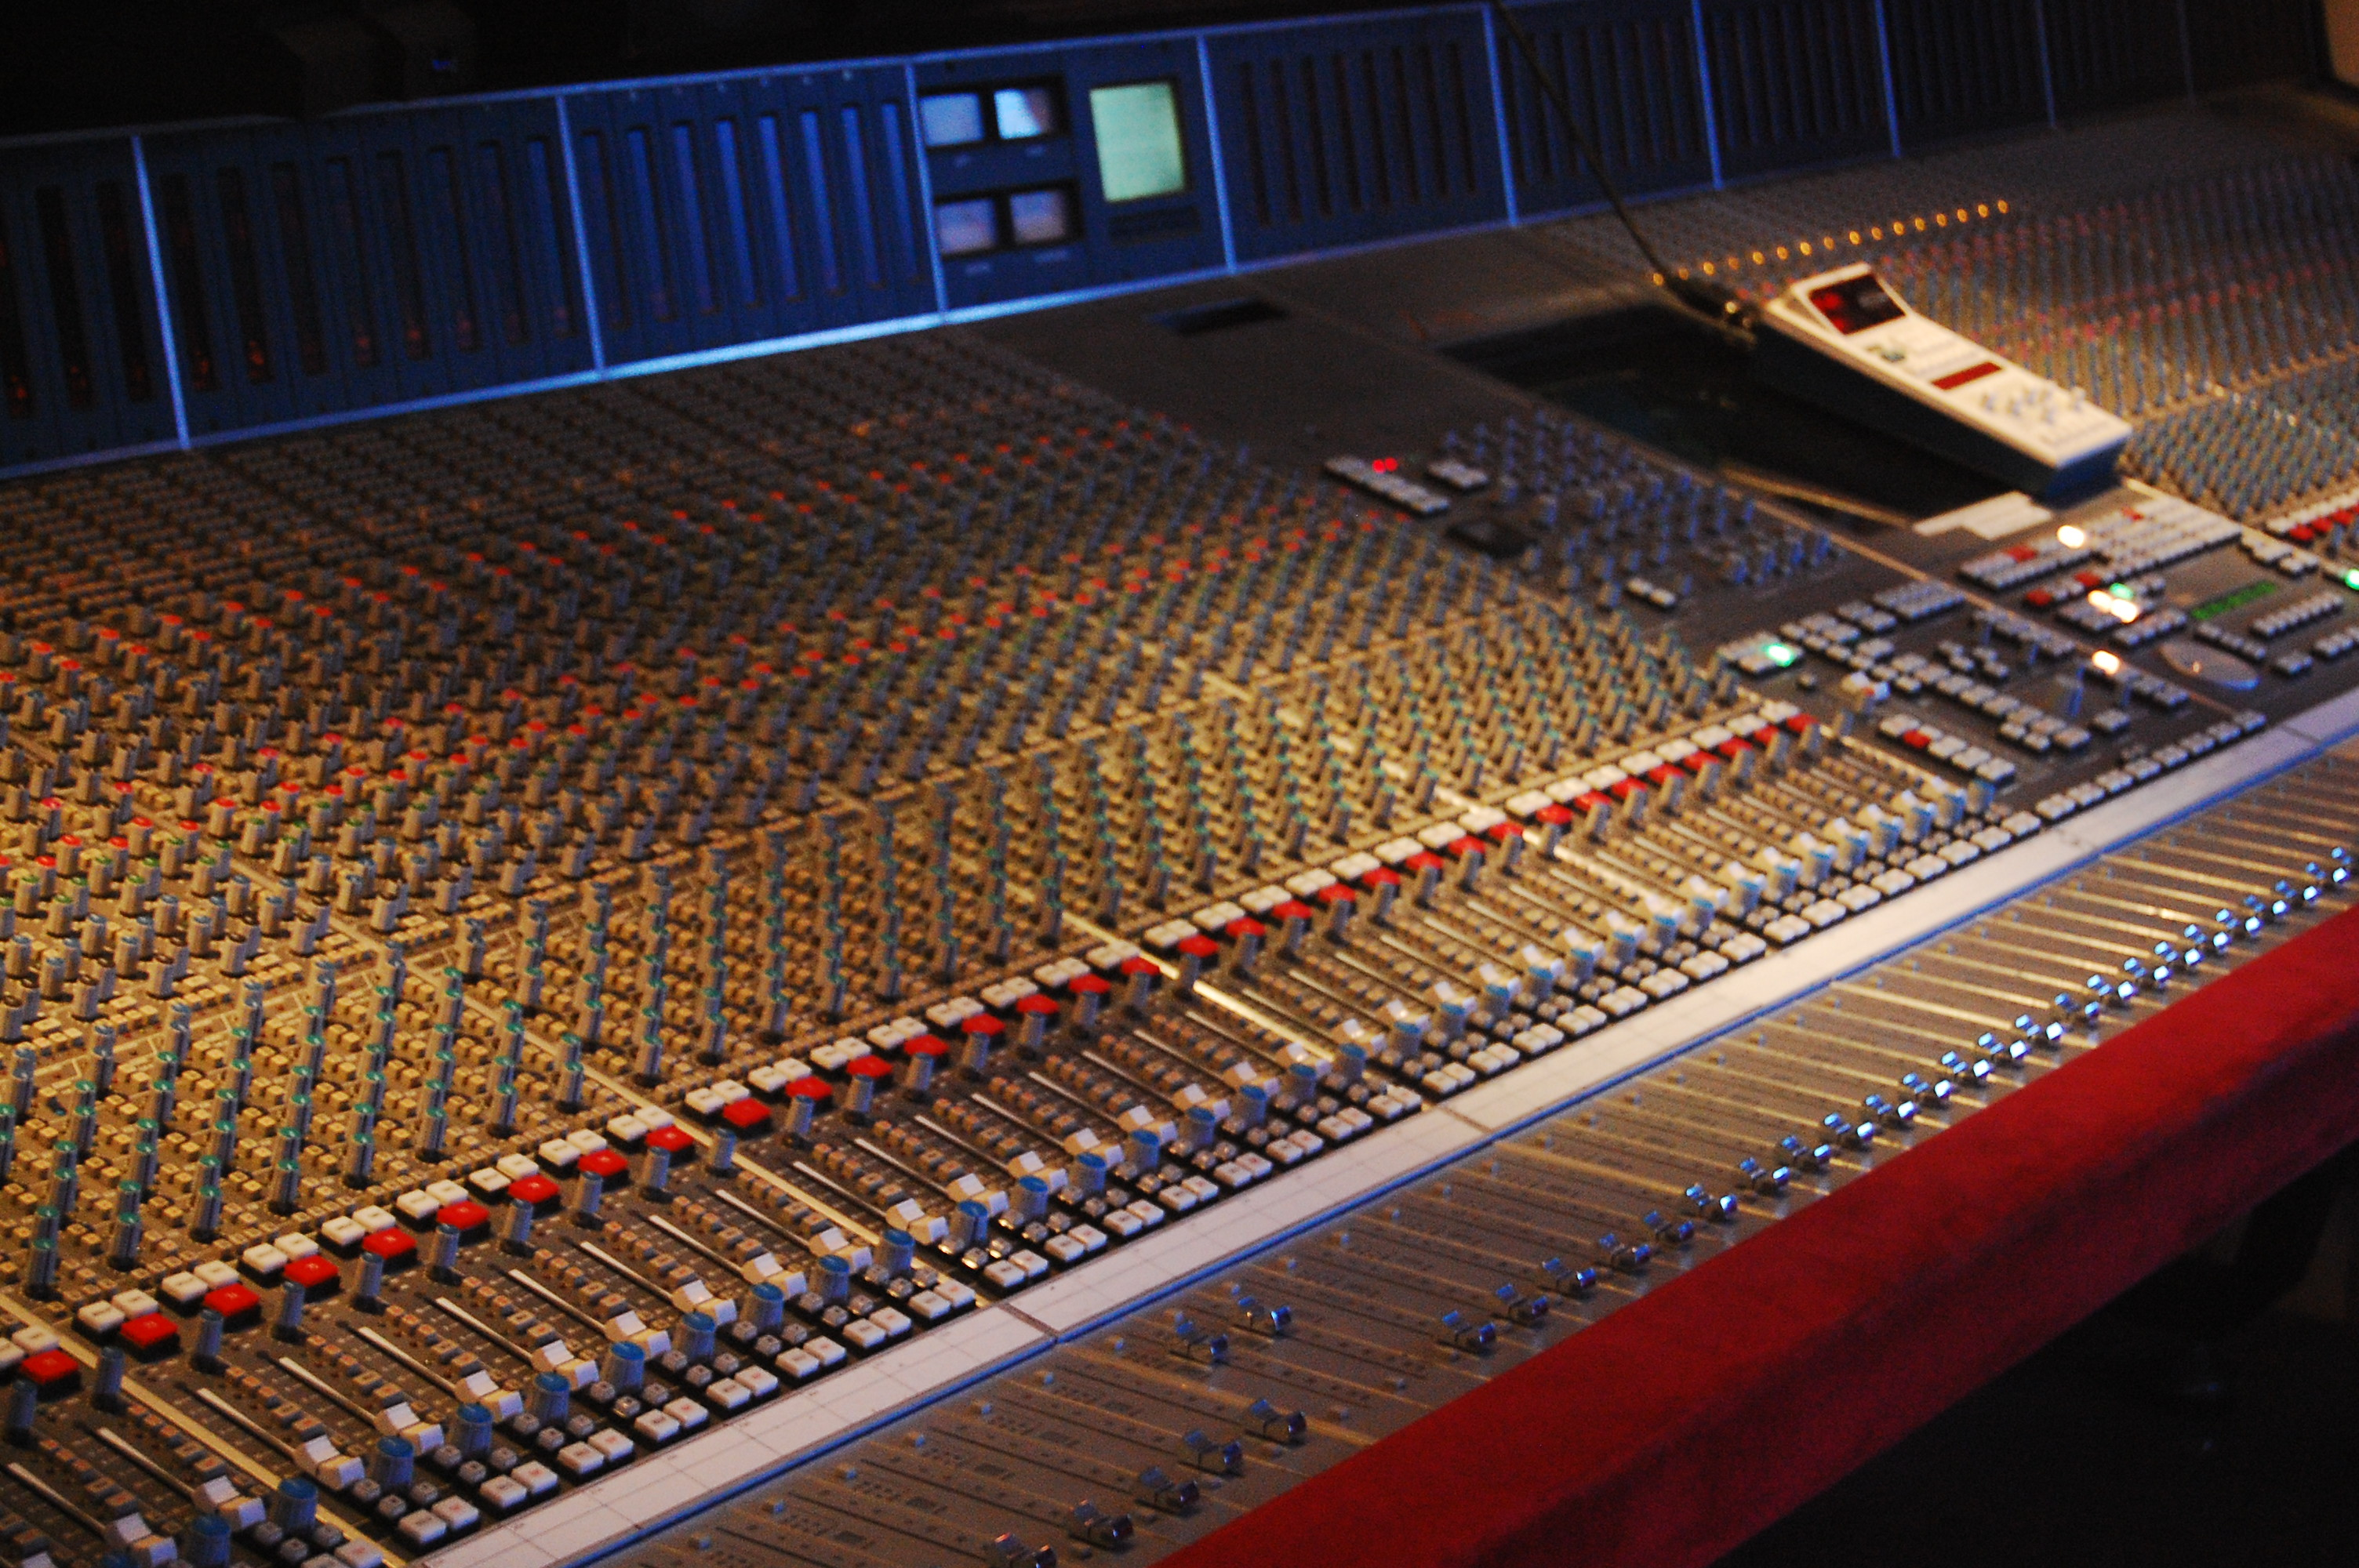
\includegraphics[scale=0.08]{miksebord.jpg}
\caption{Hvor er groove-spaken?}
\end{figure}
\end{frame}

 \begin{frame}
     \frametitle{Konklusjon}
     \begin{itemize}
         \item Metode er \emph{essensielt}.
         \item Vi må definere problemene våre på en måte som kan \emph{måles}.
         \item DTrace er et ekspertverktøy…
         \item …men kan også hjelpe oss til å \emph{bli} eksperter!
     \end{itemize}
 \end{frame}

 \begin{frame}
     \frametitle{Hvis du vil vite mer…}
     \begin{itemize}
         \item Tips, triks, ting å lese, ting å se: \url{https://github.com/cmrosenberg/}
     \end{itemize}
 \end{frame}

 \begin{frame}
     \frametitle{Kilder}
     \printbibliography{}
 \end{frame}

 % \begin{frame}
 %     \begin{itemize}
 %         \item Miksebordbildet er fra \url{http://en.wikipedia.org/wiki/Mixing\_console#mediaviewer/File:SSL\_SL9000J\_(72ch)\_@\_The\_Cutting\_Room\_Recording\_Studios,_NYC.jpg}

 %         \item Arkitekturbildet er fra \cite{dtracemanual}[s. 33].
 %     \end{itemize}
 % \end{frame}

 \begin{frame}
     \frametitle{Spørsmål?}
     \begin{itemize}
         \item Spørsmål?
     \end{itemize}
 \end{frame}

 \begin{frame}
     \frametitle{Takk for meg!}
     \begin{itemize}
         \item Takk for meg!
     \end{itemize}
 \end{frame}

\end{document}
